\documentclass[manuscript=article, journal=jceda8]{achemso}
%\documentclass[journal = jacsat]{achemso}
\usepackage{chemformula} % Formula subscripts using \ch{}
\usepackage[T1]{fontenc} % Use modern font encodings
\usepackage[utf8]{inputenc}
\usepackage[version=3]{mhchem}
\usepackage{gensymb}
\usepackage{upgreek}
\usepackage{pgfplots}
\usepackage{pst-plot}
\usepackage{tikz}
\usepgfplotslibrary{colormaps}
\usetikzlibrary{pgfplots.colormaps}
\usepgfplotslibrary{external} 
\tikzexternalize
\newcommand*\mycommand[1]{\texttt{\emph{#1}}}



\author{András Kiss}
\affiliation{Department of General and Physical Chemistry, University of Pécs, Ifjúság útja 6, 7622 Pécs, Hungary}
\email{akiss@gamma.ttk.pte.hu}
\author{János Klucsik}
\affiliation{Department of General and Physical Chemistry, University of Pécs, Ifjúság útja 6, 7622 Pécs, Hungary}
%\author{Géza Nagy}
%\affiliation{Department of General and Physical Chemistry, University of Pécs, Ifjúság útja 6, 7622 Pécs, Hungary}
\title{A simple and inexpensive pH electrode made from the tungsten filament of an incandescent light--bulb}
\keywords{pH, electrode, tungsten, light--bulb, potentiometry}



\begin{document}
\begin{abstract}
A simple and robust pH sensitive electrode is presented that can be constructed from cheap and readily available components. The electrode is of the metal/metal--oxide type. The sensing element is the tungsten filament of an incandescent light bulb, whose potential in a solution is dependent on the hydrogen--ion activity. The electrode can be easily built in a high--school chemistry laboratory by students, and can be used to demonstrate the potentiometric determination of pH.
\end{abstract}

\section{Introduction}


pH is one of the most important concepts in chemistry, originally defined by S\o rensen in 1909 \cite{sorensen1909messung} as the negative logarithm of the concentration of hydrogen ion:

\begin{equation}
\textrm{pH} = -\log_{10} c_{\textrm{H}^+}
\end{equation}

At first glance, it looks like a deceptively simple concept. Complications around this definition start to arise when we replace concentration with activity, taking into account that hydrogen ions have charge, therefore their behaviour correlates more closely with activity than concentration:

\begin{equation}
\textrm{pH} = -\log_{10} a_{\textrm{H}^+} = -\log_{10} c_{\textrm{H}^+} \gamma_{H^+}
\end{equation}

where $a_{H^+}$ is the activity and $\gamma_{H^+}$ is the activity coefficient of hydrogen ions. This definition however raises another problem. It includes the activity coefficient of a single ion, which is unmeasurable. It is possible to measure the \emph{mean activity coefficient} only, for example in the case of HCl solution:

\begin{equation}
\gamma_{H^+, Cl^-} = \sqrt{\gamma_{H^+} \gamma_{Cl^-}}
\end{equation}


Even though the Debye--Hückel equation can be used to calculate a theoretical activity coefficient for a single ion, the prevailing view is that if it cannot be measured, than a pH definition that is based on that activity coefficient is an unmeasurable quantity. This logical difficulty was summarized by Bates and Guggenheim in 1960 \cite{bates1960report}. 

Their recommended solution was a convention -- since then it has been known as the \emph{Bates--Guggenheim convention} --, in which the activity of a chosen ionic species is defined using the Debye--Hückel equation, and the rest is calculated using the theoretically obtained value for the single ionic species and the experimentally determined mean activity coefficient. The chosen ion is chloride ion. For instance, the activity coefficient of hydrogen ion can be calculated as:

\begin{equation}
\gamma_{H^+} = \frac{\gamma_{H^+, Cl^-}^2}{\gamma_{Cl^-}}
\end{equation}

This convention has been the basis for the IUPAC (International Union of Pure and Applied Chemistry) recommendation to define pH in 1985 \cite{covington1985definition} and 2002 \cite{buck2002measurement}, which is currently the most up to date definition from IUPAC:

\begin{equation}
\textrm{pH}= -\log_{10}a_{H^+} = -\log_{10}(m_{H^+} \gamma_{m, H^+}/m^\theta)
\end{equation}

where $m_{H^+}$ is the molality and $\gamma_{m, H^+}$ is the molality based activity coefficient of hydrogen ions, $m^\theta$ is the standard molality (1 mol kg$^{-1}$). The activity coefficient of hydrogen ions in the above equation is calculated using the Bates--Guggenheim convention.




The electrochemical cell used in the measurement of the primary pH standards is known as the \emph{Harned Cell} \cite{harned1958activity}.
To measure the pH in such a cell, a conventional procedure was developed at NBS (National Bureau of Standards) \cite{durst1975standardization} and recommended at present by the last IUPAC recommendations \cite{covington2002measurement}.
NIST (National Institute of Standards and Technology) in the U.S. and PTB (Physikalisch-Technische Bundesanstalt) in Germany have presented pH values using the Harned Cell. 


METHODS TO MEASURE pH
Haber and Klemensiewicz gave a full account of the response of the glass electrode in their 1909 paper \cite{haber1909elektrische, haber1909concerning}.


WHY ARE METAL/METAL-OXIDE pH ELECTRODES USEFUL
There are certain applications where the use of a glass electrode might be challenging or impossible.
These include measuring pH at high temperature or in hydrogen--fluoride solution, or application in the food industry. 

Intensive research has been conducted for several decades to find alternatives to the glass electrode. One such alternative is to use metal/metal-oxide electrodes.
One of the most often used type of these is the Ir/IrO$_2$ electrode \cite{beyenal2004improved}.
The oldest is certainly the Sb/Sb$_2$O$_3$ electrode, its initial characterization dating back to 1923 \cite{uhl1923electrometric}.
It is based on the equilibrium between antimony and the antimony-oxide on its surface.
It is pH sensitive because hydrogen ions participate in the equilibrium:

\begin{equation}
        \ce{2Sb_{(s)} + 3H_2O <=> Sb_2O_3 + 6H^+ + 6e^-}
\end{equation}

\begin{equation}
        \ce{Sb_{(s)} + 3OH^- <=> Sb(OH)_3 + 6e^-}
\end{equation}

Using the Nernst-equation to describe the relationship between [Sb$^{3+}$] and the measured electrode potential \cite{kurzweil2009metal}:

\begin{equation}
E = E^\theta - \frac{RT}{3F}\ln a_{\textrm{Sb}^{3+}}
\end{equation}

Which can be rewritten by using $K_W$, the water ion product, and $K_L$, the solubility product of antimony hydroxide as \cite{kurzweil2009metal}:

\begin{equation}
E = E^\theta - \frac{RT}{3F}\ln \frac{K_L}{K_W} + \frac{RT}{F}\ln a_{\textrm{H}^+}
= E^{\theta '} - \frac{RT}{0.4343F} \textrm{pH}  
\end{equation}
because [Sb$^{3+}$]=[H$^+$]$\cdot K_L / K_W$.

The main reason this particular electrode is so popular is that the melting point of antimony and the softening point of borosilicate glass are similar ($T_{m, \textrm{Sb}} = 630.63~\celsius$, $T_{m, glass}\approx 700~\celsius$), and manufacturing them is relatively easy with standard glass blowing techniques.

Another very popular metal/metal-oxide electrode used for pH measurements is the tungsten electrode. Its function is also based on the equilibrium between the metal and its oxide:
\begin{equation}
        \ce{W_{(s)} + 2H_2O <=> WO_2 + 4H^+ + 4e^-}
\end{equation}

TUNGSTEN ELECTRODE REACTIONS:




\begin{align}
\ce {W + 2 H2O &-> WO2 + 4 H^+ + 4 e^-}\\
\ce {W + 3 H2O &-> WO3 + 6 H^+ + 6 e^-}\\
\ce {4W + 12 H2O &-> W4O12 + 24 H^+ + 24 e^-}\\
\ce {W + 4 H2O &-> H2WO4 + 6 H^+ + 6 e^-}\\
\ce {WO2 + H2O &-> WO3 + 2 H^+ + 2 e^-}\\
\ce {WO2 + 2 H2O &-> H2WO4 + 2 H^+ + 2 e^-}
\end{align}

In this paper the construction and usage of a simple and inexpensive tungsten pH sensitive electrode is presented. The electrode can be assembled in a highschool chemistry laboratory by students and it can be used as an aid to demonstrate pH, ion-selective electrodes and metal/metal-oxide type electrodes in particular. The necessary parts can be obtained from a local hardware store or even a supermarket.


\section{Materials and Methods}


\begin{figure}[!h]
\centering
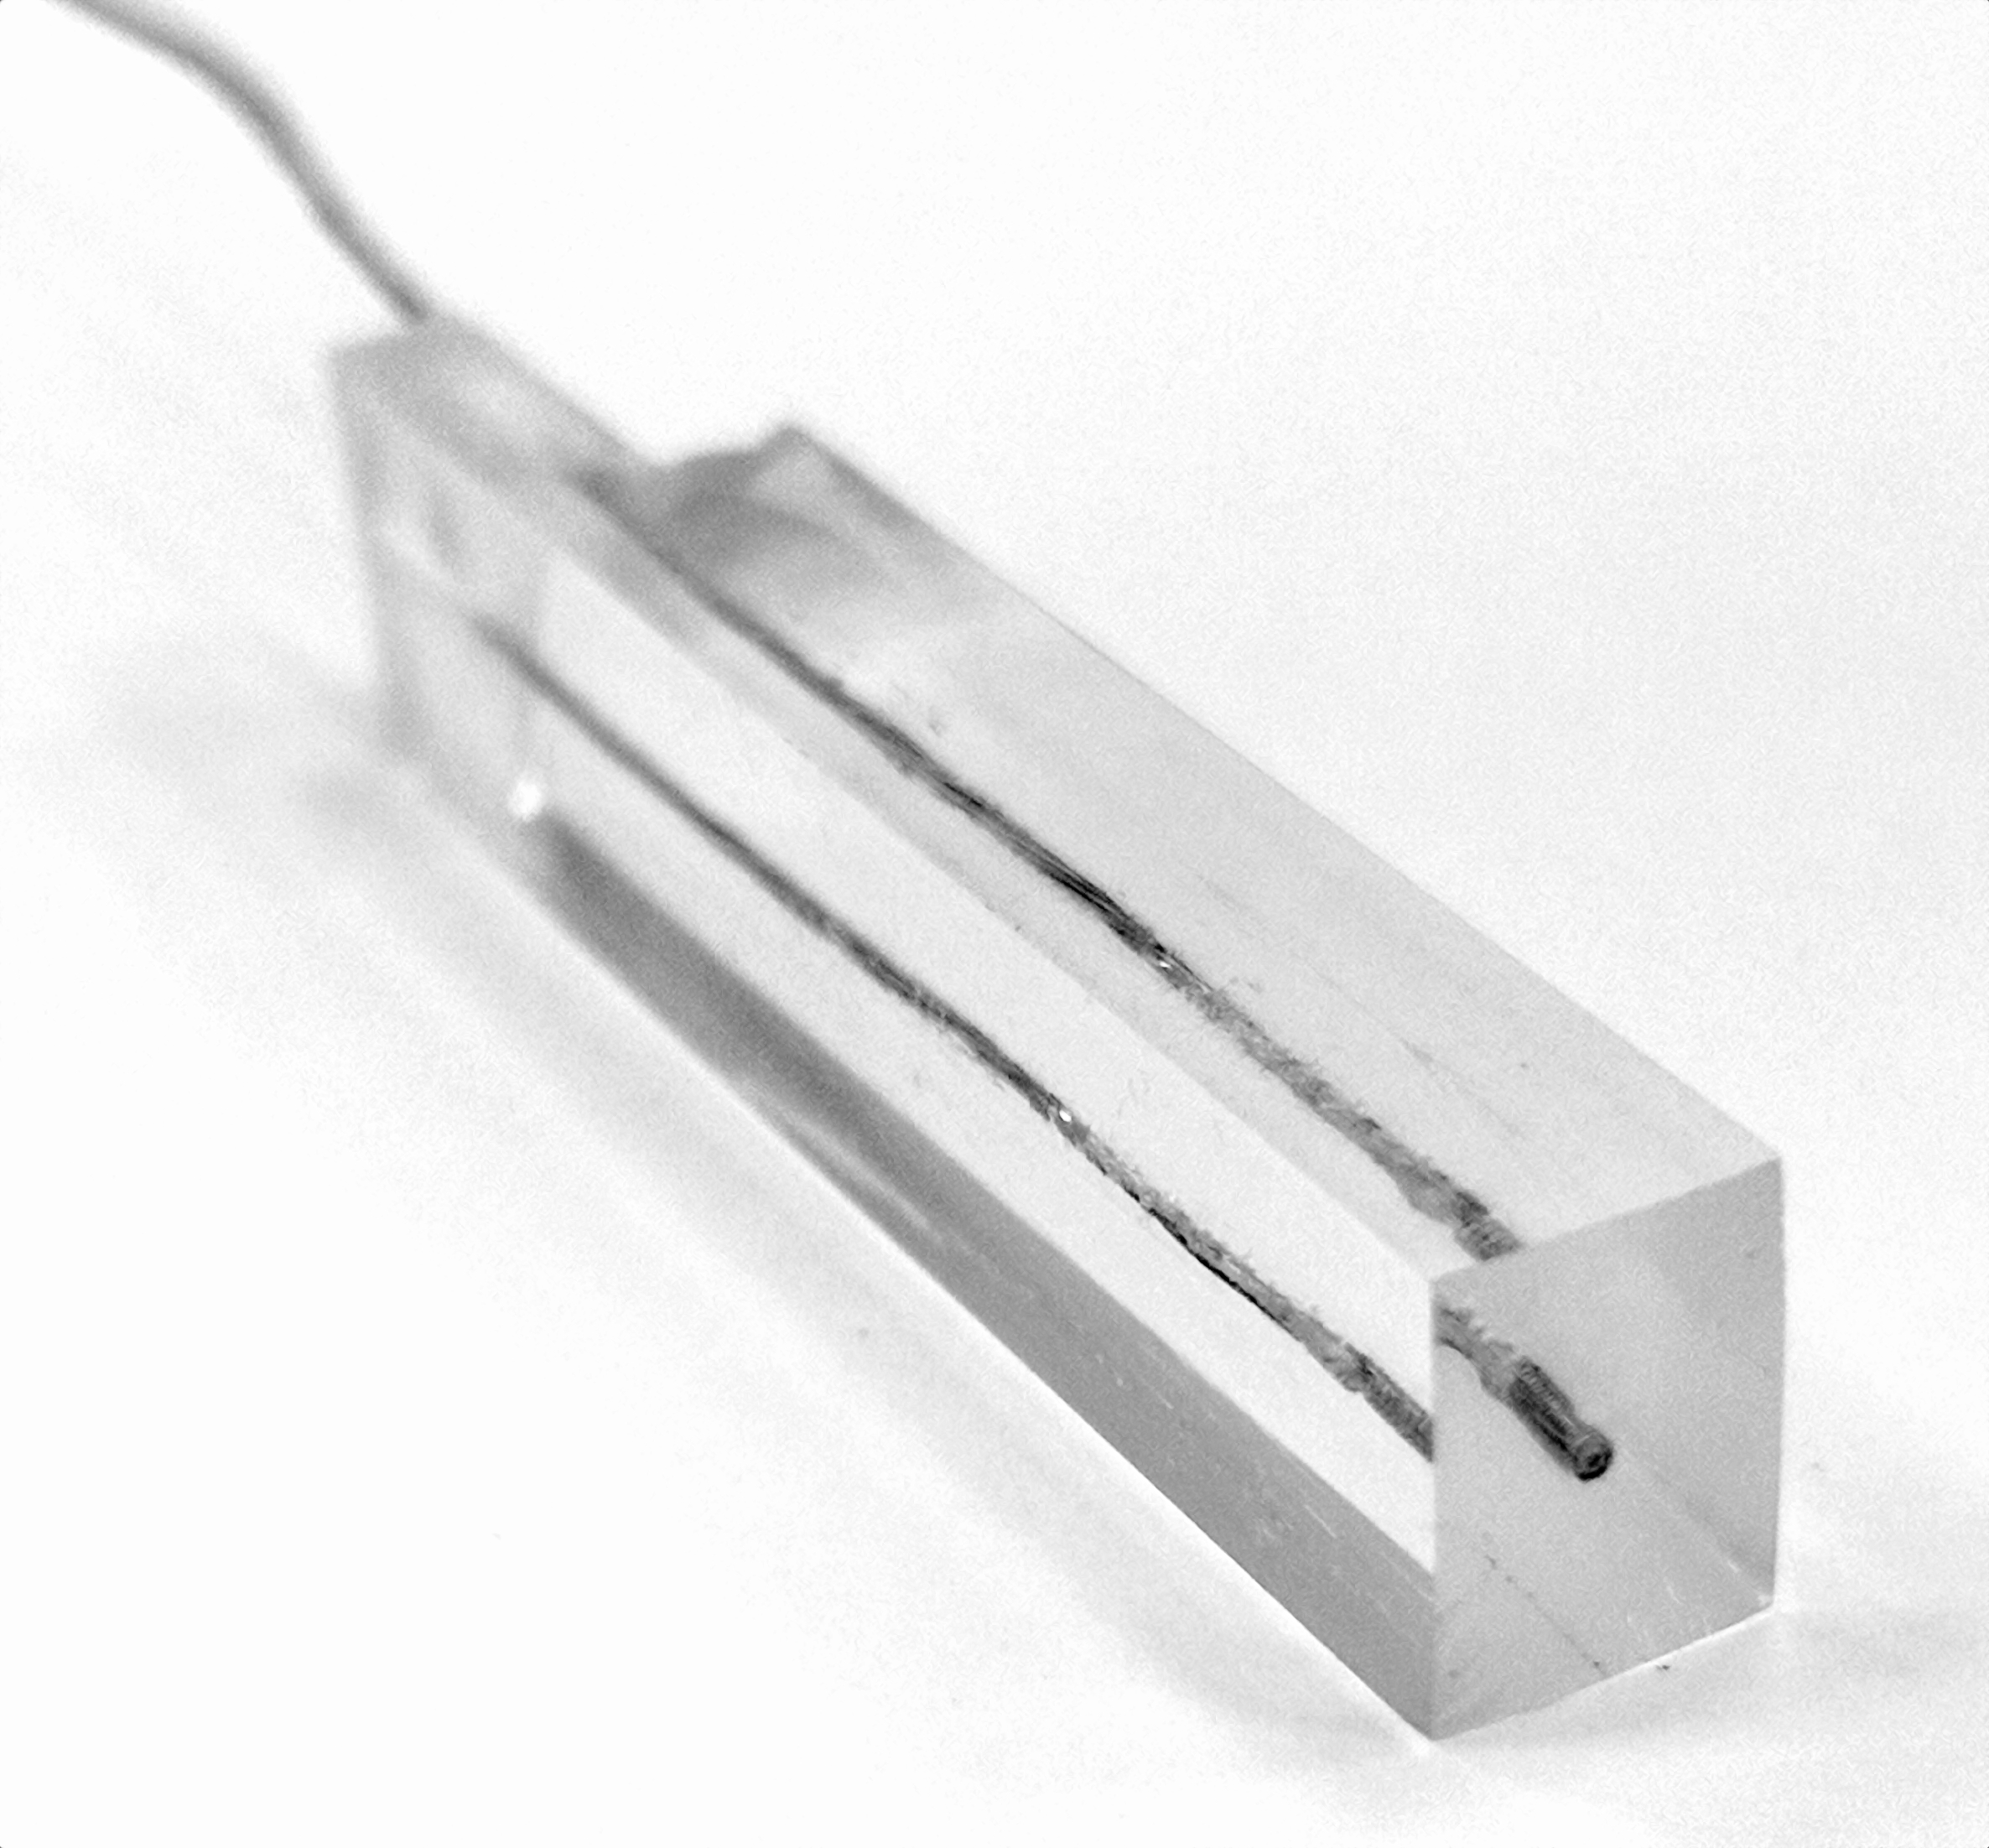
\includegraphics[width=0.5\textwidth]{img/plexi.jpg}
\caption{...}
\label{fig:plexi}
\end{figure}

Since tungsten has the highest melting point of all the elements (3422 $\celsius$), the method described in the previous paragraph cannot be used.
A tungsten microwire with a diameter of $30~\upmu$m (Element-explorer, Montreal, Canada) were sealed into a borosilicate glass capillary ($d_i=1.12~$mm, $d_o=2~$mm, no filament, World Precision Inc., Sarasota, Florida, USA).
To seal the microwire, one end of the capillary was closed with flame.
Then, a 1$~$cm long tungsten microwire was inserted from the other end, and pushed down to the sealed end.
The sealed end was melted again while vacuum was being applied from the open end.
The capillary was kept in the flame until $4-5~$mm, about half of the microwire was sealed into the glass.
To make electrical contact between the microwire and the measuring instruments, a small piece of solder was inserted into the capillary.
The solder was melted in flame, and pushed down to the sealed end of the capillary by a sudden shake of the wrist.
While the solder was still melted, a copper wire was insterted into the solder.
After the solder had cooled down, the electrodes were ready to be used.
Microelectrodes with $30~\upmu$m tungsten filaments from a 100$~$W Tungsram incandescent lightbulb were also prepared, using the same method.




\section{Results}

\begin{figure}
\centering
\begin{tikzpicture}
\begin{axis}	[
		%legend style={draw=none},
		legend style={draw=none, at={(0.5,0.98)}, anchor=north},
		%legend style=draw=none, at={(0.5,-0.1)}, anchor=north
		xmin=0,
		xmax=3060,
		ymin=-400,
		ymax=200,
		width=12cm,
		height=8cm,
		xlabel=t / s,
		ylabel=E vs. Ag/AgCl/KCl(3 M) / mV
		%ytick={-0.31, -0.3, -0.29, -0.28, -0.27},
		%/pgf/number format/.cd, use comma, 1000 sep={}
		]
\addplot [color=blue] table {data/calibration/uveg.txt};
\addplot [color=red] table {data/calibration/sigma.txt};
\addplot [color=green] table {data/calibration/izzo.txt};
\addlegendentry{Üvegelektród}
\addlegendentry{Volfrámelektród}
\addlegendentry{Izzószálelektród}
%\node[anchor=north west] at (rel axis cs:0.02,0.98) {A};
\end{axis}
\end{tikzpicture}
\caption{A két volfrám mikroelektród kalibrációs mérései. Összehasonlításképpen egy üvegelektród egyidejűleg mért potenciál--idő mérését is ábrázoltam. A potenciált mindhárom elektród esetében az üvegelektród belső, Ag/AgCl/KCl (3 M) referencia félcellájához képest mértem egy kellően nagy bemeneti impedanciájú feszültségmérő (eDAQ isopod EPU) felhasználásával.}
\label{fig:kalibracios_meres}
\end{figure}



\begin{figure}[h!]
\centering
\begin{tikzpicture}
\begin{axis}[
legend style={draw=none, at={(0.02,0.98)}, anchor=north west},
	xmin=0.5, xmax=10, width=7cm,height=7cm,xlabel=pKATION, ylabel={E vs. Ag/AgCl/KCl(3 M), mV}, clip marker paths=true, xtick = {0,1,2,3,4,5,6,7,8,9,10}, xminorticks=true, minor x tick num = 1]
\addplot [only marks, domain=0:5.5, mark=*, color=red] table {data/calibration/uveg_h.txt};
\addplot [only marks, domain=0:5.5, mark=*, color=blue] table {data/calibration/uveg_na.txt};
\addplot [only marks, domain=0:5.5, mark=*, color=green] table {data/calibration/uveg_k.txt};
\addplot [only marks, domain=0:5.5, mark=*, color=black] table {data/calibration/uveg_mg.txt};
\addplot [only marks, domain=0:5.5, mark=*, color=purple] table {data/calibration/uveg_ca.txt};
%\addplot [domain=0:3, samples=500, line width=0.1mm] {86.8-x*29.12};
\addlegendentry{H$^+$} 
\addlegendentry{Na$^+$}
\addlegendentry{K$^+$}
\addlegendentry{Mg$^{2+}$}
\addlegendentry{Ca$^{2+}$}
\node[anchor=north east] at (rel axis cs:0.98,0.98) {A};
\node[anchor=south west] at (rel axis cs:0,0) {$\Delta$ S = 54.788 mV / pH};
\node[anchor=south west] at (rel axis cs:0,0.1) {R$^2$ = 0.9998};
\end{axis}
\end{tikzpicture}
\begin{tikzpicture}
\begin{axis}[
legend style={draw=none, at={(0.02,0.98)}, anchor=north west},
xmin=0.5, xmax=10, width=7cm,height=7cm,xlabel=pKATION, ylabel={E vs. Ag/AgCl/KCl(3 M), mV}, clip marker paths=true, xtick = {0,1,2,3,4,5,6,7,8,9,10}, xminorticks=true, minor x tick num = 1]
\addplot [only marks, domain=0:5.5, mark=*, color=red] table {data/calibration/sigma_h.txt};
\addplot [only marks, domain=0:5.5, mark=*, color=blue] table {data/calibration/sigma_na.txt};
\addplot [only marks, domain=0:5.5, mark=*, color=green] table {data/calibration/sigma_k.txt};
\addplot [only marks, domain=0:5.5, mark=*, color=black] table {data/calibration/sigma_mg.txt};
\addplot [only marks, domain=0:5.5, mark=*, color=purple] table {data/calibration/sigma_ca.txt};
%\addplot [domain=0:3, samples=500, line width=0.1mm] {86.8-x*29.12};
\addlegendentry{H$^+$} 
\addlegendentry{Na$^+$}
\addlegendentry{K$^+$}
\addlegendentry{Mg$^{2+}$}
\addlegendentry{Ca$^{2+}$}
\node[anchor=north east] at (rel axis cs:0.98,0.98) {B};
\node[anchor=south west] at (rel axis cs:0,0) {$\Delta$ S = 51.157 mV / pH};
\node[anchor=south west] at (rel axis cs:0,0.1) {R$^2$ = 0.9986};
\end{axis}
\end{tikzpicture}

\begin{tikzpicture}
\begin{axis}[
	legend style={draw=none, at={(0.02,0.98)}, anchor=north west},
	xmin=0.5, xmax=10,
	width=7cm,height=7cm,
	xlabel=pKATION, ylabel={E vs. Ag/AgCl/KCl(3 M), mV},
	clip marker paths=true,
	xtick = {0,1,2,3,4,5,6,7,8,9,10}, xminorticks=true, minor x tick num = 1]
\addplot [only marks, domain=0:5.5, mark=*, color=red] table {data/calibration/izzo_h.txt};
\addplot [only marks, domain=0:5.5, mark=*, color=blue] table {data/calibration/izzo_na.txt};
\addplot [only marks, domain=0:5.5, mark=*, color=green] table {data/calibration/izzo_k.txt};
\addplot [only marks, domain=0:5.5, mark=*, color=black] table {data/calibration/izzo_mg.txt};
\addplot [only marks, domain=0:5.5, mark=*, color=purple] table {data/calibration/izzo_ca.txt};
%\addplot [domain=0:3, samples=500, line width=0.1mm] {86.8-x*29.12};
\addlegendentry{H$^+$} 
\addlegendentry{Na$^+$}
\addlegendentry{K$^+$}
\addlegendentry{Mg$^{2+}$}
\addlegendentry{Ca$^{2+}$}
\node[anchor=north east] at (rel axis cs:0.98,0.98) {C};
\node[anchor=south west] at (rel axis cs:0,0) {$\Delta$ S = 53.207 mV / pH};
\node[anchor=south west] at (rel axis cs:0,0.1) {R$^2$ = 0.9817};
\end{axis}
\end{tikzpicture}
\caption{(A) Üvegleketród (B) volfrámelektród (C) izzószálelektród kalibrációs egyenese, illetve szelektivitás-vizsgálata.}
\label{fig:kalibracios_egyenes}
\end{figure}

		
\begin{acknowledgement}
The author thanks Mats Dahlgren for version one of \textsf{achemso},
\end{acknowledgement}

\bibliography{tungsten}
\end{document}
